\chapter{HASIL DAN PEMBAHASAN}
\label{chap:hasildanpembahasan}

\section{Hasil Eksperimen}
\label{sec:hasilpengujian}

Pada bagian ini, kami akan membahas hasil eksperimen yang dilakukan
untuk menjawab rumusan masalah yang diajukan dalam penelitian ini.

\subsection{Lingkungan Pengujian}
\label{subsec:lingkunganpengujian}

Untuk menjawab rumusan masalah yang diajukan oleh penelitian ini,
kami melakukan eksperimen pada aplikasi \emph{benchmark}
DISC yang telah ada, yang diadaptasi dari penelitian sebelumnya
tentang \emph{debugging} dan pengujian aplikasi DISC. \emph{Benchmark}
ini merupakan campuran dari alur kerja \emph{big data} yang
terinspirasi dari SQL dan dunia nyata. Aplikasi-aplikasi
ini juga dilengkapi dengan kesalahan yang sudah disuntikkan
sebelumnya yang mewakili \emph{bug} dunia nyata. Secara total,
kami menjalankan eksperimen pada 16 aplikasi \emph{benchmark}
DISC yang bermasalah. Aplikasi-aplikasi ini dilengkapi
dengan skrip pembuatan data yang memungkinkan data
dihasilkan dengan faktor skala, mirip dengan
\emph{benchmark} TPC-DS. Kami menggunakan laptop standar
untuk menerapkan Apache Spark 2.0.0 karena Titian
awalnya dirancang untuk Apache Spark 2.0.0. Namun,
FISUM sepenuhnya kompatibel dengan versi terbaru dari
Spark karena tidak memerlukan instrumen apa pun dalam
kode sumber Apache Spark. 

Berikut adalah deskripsi dari ke 16 aplikasi \emph{benchmark}
yang digunakan dalam penelitian ini:
\begin{enumerate}
      \item \emph{\textbf{Age Analysis}} \\
            Program \emph{age analysis} digunakan untuk mengklasifikasikan penduduk di sebuah area dengan kode pos "90024" sesuai dengan umur mereka. 
            Dalam program ini, Titian diaplikasikan untuk mendeteksi input yang memiliki data penduduk yang memiliki umur lebih dari 50 atau kode pos nya adalah "null".
            Adapun contoh dataset yang digunakan dapat 
            dilihat pada \ref{tb:ageanalysisdataset}.

            \begin{longtable}{|c|c|c|}
                  \caption{Contoh Dataset Age Analysis.}
                  \label{tb:ageanalysisdataset} \\
                  \hline
                  \rowcolor[HTML]{C0C0C0}
                  \textbf{Kode Pos} & \textbf{Umur} & \textbf{Jumlah} \\
                  \hline
                  90024 & 20 & 1000 \\
                  null & 30 & 2000 \\
                  90024 & 159 & 3000 \\
                  \hline
            \end{longtable}
      
      \item \emph{\textbf{Commute Type}} \\
            Program \emph{commute type} menggunakan dataset berupa kode pos area A, kode pos area B, jarak, serta waktu yang ditempuh. Selanjutnya, program akan mengolah jarak dan waktu menjadi kecepatan yang terjadi dalam menempuh perjalanan dari area A ke B. Dari data kecepatan tersebut, program akan mengklasifikasikan ke dalam tiga kategori, yaitu sebagai berikut:
            \begin{itemize}
                  \item kecepatan $ > $ 40 = \emph{car}
                  \item kecepatan $ > $ 15 = \emph{public}
                  \item kecepatan $ \leq $ 15 = \emph{on foot}
            \end{itemize}
            Namun, dari ketiga kategori tersebut, untuk kecepatan $ > $ 100 dikategorikan sebagai kesalahan input karena mobil tidak akan melebihi batas kecepatan tersebut atau jarak yang $ < $ dari 0.
            Adapun contoh dataset yang digunakan dapat 
            dilihat pada \ref{tb:commutetypedataset}.

            \begin{longtable}{|c|c|c|c|c|}
                  \caption{Contoh Dataset Commute Type.}
                  \label{tb:commutetypedataset} \\
                  \hline
                  \rowcolor[HTML]{C0C0C0}
                  \textbf{\#} & \textbf{Kode Pos A} & \textbf{Kode Pos B} & \textbf{Jarak} & \textbf{Kecepatan} \\
                  sr & 90002 & 90017 & -20 & 100 \\
                  sr & 90098 & 90077 & 2106 & 37 \\
                  sr & 90079 & 90009 & 7009 & 116 \\
                  \hline
            \end{longtable}

      \item \emph{\textbf{Commute Type Full}} \\
      

            Program \emph{commute type full} menggunakan 2 dataset, 
            yaitu \emph{trips} dan \emph{locations}. Dataset 
            \emph{trips} berupa kode pos area A, kode pos area B, 
            jarak, serta waktu yang ditempuh. Sedangkan, dataset 
            kedua yang digunakan adalah \emph{locations}, dataset 
            ini berisi lokasi dari sebuah kode pos. Selanjutnya, 
            program akan menggabungkan kedua dataset apabila ada 
            kesamaan pada kode pos. Kemudian, program akan mengolah 
            jarak dan waktu menjadi kecepatan yang terjadi dalam 
            menempuh perjalanan dari kota A ke B. Dari data kecepatan 
            tersebut, program akan mengklasifikasikan ke dalam tiga 
            kategori, yaitu sebagai berikut:
            \begin{itemize}
                  \item kecepatan $ > $ 40 = \emph{car}
                  \item kecepatan $ > $ 15 = \emph{public}
                  \item kecepatan $ \leq $ 15 = \emph{on foot}
            \end{itemize}
            Pada program ini, Titian bekerja untuk mendeteksi input yang dianggap salah, yaitu yang memiliki ID lokasi kurang dari sama dengan 1000 atau Country yang bernilai "Null".
            Adapun contoh dataset yang digunakan dapat 
            dilihat pada \ref{tb:commutetypefulldataset}.
            % 610,18.2911,-67.12243,Anasco,PR,Puerto Rico,TRUE,,26502,275.7,72011,Añasco,,Añasco|Moca|Las Marías|Aguada,72011|72099|72083|72003,FALSE,FALSE,America/Puerto_Rico
            % 611,18.27698,-66.80688,Angeles,PR,Puerto Rico,TRUE,,,,72141,Utuado,,Utuado,72141,FALSE,FALSE,America/Puerto_Rico
            % 612,18.41283,-66.7051,Arecibo,PR,Puerto Rico,TRUE,,58771,298,72013,Arecibo,,Arecibo|Hatillo|Barceloneta,72013|72065|72017,FALSE,FALSE,America/Puerto_Rico
            
            
            \begin{longtable}{|c|c|c|c|c|}
                  \caption{Contoh Dataset Commute Type Full.}
                  \label{tb:commutetypefulldataset} \\
                  \hline
                  \rowcolor[HTML]{C0C0C0}
                  \textbf{ID} & \textbf{Latitude} & \textbf{Longitude} & \textbf{City} & \textbf{State}\\
                  \hline
                  610 & 18.2911 & -67.12243 & Anasco & PR \\
                  611 & 18.27698 & -66.80688 & Angeles & PR \\
                  \hline
                  \rowcolor[HTML]{C0C0C0}
                  \textbf{Country} & \textbf{IsPrimary} & \textbf{Zip} & \textbf{CountyName} & \textbf{CountyANSI}\\
                  \hline
                  Null & TRUE & 26502 & Añasco & 72011 \\
                  Puerto Rico & TRUE & 72141 & Utuado & 72141 \\

                  \hline
                  \rowcolor[HTML]{C0C0C0}
                  \textbf{Cities} & \textbf{CitiesFIPS} & \textbf{IsCSAS} & \textbf{IsMSAS} & \textbf{TimeZone}\\
                  \hline
                  Añasco \textbar{} Moca  & 72011 \textbar{} 72099  & FALSE & FALSE & America/Puerto\_Rico \\
                  Utuado & 72141 & FALSE & FALSE & America/Puerto\_Rico \\
                  \hline
            \end{longtable}

      \

      \
      \item \emph{\textbf{Customers}} \\
      % s"""$oid,$cid,$time,$item"""
      % order651,888,78895039,item797864327
      % order515,481,1701910512,item765935155
      % order531,24,1171869537,item354502894
            Program \emph{customers} akan mengolah dua dataset, yaitu dataset \emph{customers\_data} dan \emph{orders\_data}. Kedua dataset ini akan digabungkan apabila memiliki kesamaan data dan akan menganalisis customer mana yang setidaknya sudah membuat 3 kali pembelian dalam jangka waktu yang sudah ditentukan. Dalam program ini, Titian hanya mencari input data yang memiliki order ID kurang dari 100 atau waktu yang $ < $ 0 dan dinyatakan sebagai input yang salah.
            Adapun contoh dataset yang digunakan dapat 
            dilihat pada \ref{tb:customersdataset}.

            \begin{longtable}{|c|c|c|c|}
                  \caption{Contoh Dataset Customers.}
                  \label{tb:customersdataset} \\
                  \hline
                  \rowcolor[HTML]{C0C0C0}
                  \textbf{ID Order} & \textbf{ID Pelanggan} & \textbf{Waktu} & \textbf{Item} \\
                  \hline
                  order651 & 888 & 78895039 & item797864327 \\
                  order515 & 481 & -20 & item765935155 \\
                  order531 & 24 & 1171869537 & item354502894 \\
                  \hline
            \end{longtable}
            
      \item \emph{\textbf{Delays}} \\
      % s"""$tripId,$a,$d,$r"""
      % trip63811,2128804415,1221732780,route56
      % trip46102,1777873050,482274628,route49
      % trip38403,140174683,1960456261,route64
            \emph{Delays} adalah program yang digunakan untuk mencari data bus yang mengalami keterlambatan (\emph{delay}). Dataset yang digunakan ada 2, yaitu \emph{dataStation1} dan \emph{dataStation2}. Kedua dataset ini memiliki waktu keberangkatan dan tiba dari setiap ID perjalanan. Kemudian, kedua dataset digabungkan apabila memiliki kesamaan data. Selanjutnya, program akan menghitung keterlambatan dari waktu keberangkatan dan tiba dari setiap elemen. Dalam program ini, Titian diterapkan untuk mencari input data yang memiliki waktu keberangkatan lebih besar daripada waktu tiba, karena dinyatakan sebagai ketidakmungkinan dalam kasus nyata atau id perjalanan yang bernilai "Null".
            Adapun contoh dataset yang digunakan dapat 
            dilihat pada \ref{tb:delaysdataset}.

            \begin{longtable}{|c|c|c|c|}
                  \caption{Contoh Dataset Delays.}
                  \label{tb:delaysdataset} \\
                  \hline
                  \rowcolor[HTML]{C0C0C0}
                  \textbf{ID Perjalanan} & \textbf{Waktu Berangkat} & \textbf{Waktu Tiba} & \textbf{Rute} \\
                  \hline
                  trip63811 & 2128804415 & 1221732780 & route56 \\
                  null & 1777873050 & 482274628 & route49 \\
                  trip38403 & 140174683 & 1960456261 & route64 \\
                  \hline
            \end{longtable}

      \item \emph{\textbf{Delivery Faults}} \\
      % s"""$did,$cid,$vend,$rating"""
      % dlvry96998,cust43114,vend65077,5
      % dlvry16209,cust64119,vend8516,5
      % dlvry89647,cust10882,vend3328,5
            \emph{Delivery Faults} adalah program yang dapat mencari pengiriman mana yang buruk dari rating yang dimilikinya. Titian diterapkan dalam program ini untuk mendeteksi input yang memiliki rating lebih dari 5 atau id pengiriman bernilai "null".
            Adapun contoh dataset yang digunakan dapat 
            dilihat pada \ref{tb:deliveryfaultsdataset}.

            \begin{longtable}{|c|c|c|c|}
                  \caption{Contoh Dataset Delivery Faults.}
                  \label{tb:deliveryfaultsdataset} \\
                  \hline
                  \rowcolor[HTML]{C0C0C0}
                  \textbf{ID Pengiriman} & \textbf{ID Pelanggan} & \textbf{ID Vendor} & \textbf{Rating} \\
                  \hline
                  dlvry96998 & cust43114 & vend65077 & 5 \\
                  null & cust64119 & vend8516 & 5 \\
                  dlvry89647 & cust10882 & vend3328 & 5 \\
                  \hline
            \end{longtable}

      \

      \item \emph{\textbf{External Call}} \\
      % Teks
      % This is a sentence
      % This not a sentence
      % This is a word
      % My name is black
      % I am a student
            Program \emph{external call} memiliki tujuan untuk mencari kata yang sering muncul dalam suatu dataset, cara kerjanya adalah menjumlahkan setiap kata yang sama, kemudian apabila kata tersebut muncul lebih dari 1 maka dinyatakan sebagai kata yang sering muncul. Dalam program ini, Titian hanya akan melacak data yang jarang muncul yaitu yang memiliki jumlah kemunculan kurang dari atau sama dengan 1 atau bernilai "null".
            Adapun contoh dataset yang digunakan dapat 
            dilihat pada \ref{tb:externalcalldataset}.

            \begin{longtable}{|c|}
                  \caption{Contoh Dataset External Call.}
                  \label{tb:externalcalldataset} \\
                  \hline
                  \rowcolor[HTML]{C0C0C0}
                  \textbf{Teks} \\
                  \hline
                  This is a sentence \\
                  This not a sentence \\
                  null \\
                  My name is black \\
                  \hline
            \end{longtable}

      \item \emph{\textbf{Find Salary}} \\
      % $522224
      % $415728
      % $501565
      % $820638
            \emph{Find salary} menggunakan satu data set yang berisi nominal gaji setiap orang, Program ini akan mencari gaji yang kurang dari 300. Kemudian, Titian diterapkan hanya untuk mendeteksi gaji yang lebih besar atau sama dengan 300 atau bernilai "null".
            Adapun contoh dataset yang digunakan dapat 
            dilihat pada \ref{tb:findsalarydataset}.

            \begin{longtable}{|c|}
                  \caption{Contoh Dataset Find Salary.}
                  \label{tb:findsalarydataset} \\
                  \hline
                  \rowcolor[HTML]{C0C0C0}
                  \textbf{Gaji} \\
                  \hline
                  \$522224 \\
                  \$415728 \\
                  null \\
                  \hline
            \end{longtable}

      \item \emph{\textbf{Flight Distance}} \\
      % s"""$airportCode,$airportName,$airportName2,$long,$lat,$continent"""
      % LAX,2n8Hga8ICV,MpQ4TQZrHs,151.3466,-68.5339,PRkqAcg4rZ
      % LAS,hOvx8HlmGI,ke7IhMxWmx,123.0983,5.819,zQ6Zrv9bgQ
      % LAS,AJSAZYp44p,lJW9lm2npx,135.2637,-25.0603,Fter9EB1Vd
      % LAS,3L4mwHv6Wr,pkUt6axm1Y,176.4615,23.2344,wcb4CeYYo7
      % LAS,eRUZDr9FqE,XXuxIq7gGT,-134.0949,10.8214,SxtFuOA1xS
            Program \emph{flight distance} adalah program yang dapat mengolah data dari dua dataset, yaitu \emph{flights\_data} dan \emph{airports\_data}, yang mana hasil akhirnya adalah akan mengetahui jarak dari keberangkatan dan tiba dari setiap penerbangan. 
            Terdapat banyak input yang berupa lokasi bandara, kami gunakan input yang memiliki lokasi berkode "LAS" dan "LAX" sebagai input yang salah atau benua dengan nilai "null". Kemudian, input tersebut akan dilacak dengan Titian.
            Adapun contoh dataset yang digunakan dapat 
            dilihat pada \ref{tb:flightdistancedataset}.

            \begin{longtable}{|p{0.12\linewidth}|p{0.17\linewidth}|p{0.17\linewidth}|c|c|c|}
                  \caption{Contoh Dataset Flight Distance.}
                  \label{tb:flightdistancedataset} \\
                  \hline
                  \rowcolor[HTML]{C0C0C0}
                  \raggedright{\textbf{Kode Bandara}} & \raggedright{\textbf{Nama Bandara Asal}} & \raggedright{\textbf{Nama Bandara Tujuan}} & \textbf{Long} & \textbf{Lat} & \textbf{Benua} \\
                  \hline
                  LAX & 2n8Hga8ICV & MpQ4TQZrHs & 151.3466 & -68.5339 & PRkqAcg4rZ \\
                  LAS & hOvx8HlmGI & ke7IhMxWmx & 123.0983 & 5.819 & zQ6Zrv9bgQ \\
                  LAS & AJSAZYp44p & lJW9lm2npx & 135.2637 & -25.0603 & null \\
                  LAS & 3L4mwHv6W & pkUt6axm1Y & 176.4615 & 23.2344 & wcb4CeYYo7 \\
                  \hline
            \end{longtable}
      
            \
      
      
            
      \item \emph{\textbf{Income Aggregation}} \\
      % \item  s"""$zip,$age,$r"""
      % 90084,11,9248
      % 90080,12,6140
      % 90014,15,1199
      % 90031,53,7558
      % 90017,17,7820
            \emph{Income aggregation} menggunakan dataset yang terdiri dari kode pos, umur, dan jumlah income. Program ini digunakan untuk mengklasifikasikan income masing-masing orang dari umurnya. Lalu, Titian akan digunakan untuk melacak asal usul data yang memiliki kode pos 90024 atau umur $ < $ 0.
            Adapun contoh dataset yang digunakan dapat 
            dilihat pada \ref{tb:incomeaggregationdataset}.

            \begin{longtable}{|c|c|c|}
                  \caption{Contoh Dataset Income Aggregation.}
                  \label{tb:incomeaggregationdataset} \\
                  \hline
                  \rowcolor[HTML]{C0C0C0}
                  \textbf{Kode Pos} & \textbf{Umur} & \textbf{Pendapatan} \\
                  \hline
                  90024 & 11 & 9248 \\
                  90080 & 12 & 6140 \\
                  90014 & 15 & 1199 \\
                  90031 & 53 & 7558 \\
                  90017 & -22 & 7820 \\
                  \hline
            \end{longtable}

      \item \emph{\textbf{Inside Circle}} \\
      % s"""$x,$y,$r"""
      % 49,26,711
      % 7,26,1870
      % 79,62,845
      % 64,65,1768
      % 2,45,611
            \emph{Inside circle} digunakan untuk menghitung data 3 bilangan random untuk memastikan apakah bilangan x dan y ada dalam radius z. Kegagalan atau kesalahan input yang akan dicari dalam program ini adalah data yang memiliki ukuran x dan y yang berada di luar radius z, yang mana tidak ada di dalam lingkaran atau radius yang bernilai $ < $ 0.
            Adapun contoh dataset yang digunakan dapat 
            dilihat pada \ref{tb:insidecircledataset}.

            \begin{longtable}{|c|c|c|}
                  \caption{Contoh Dataset Inside Circle.}
                  \label{tb:insidecircledataset} \\
                  \hline
                  \rowcolor[HTML]{C0C0C0}
                  \textbf{X} & \textbf{Y} & \textbf{Radius} \\
                  \hline
                  49 & 26 & 711 \\
                  7 & 26 & 1870 \\
                  79 & 62 & 845 \\
                  64 & 65 & 1768 \\
                  2 & 45 & -20 \\
                  \hline
            \end{longtable}

      \item \emph{\textbf{Loan Type}} \\
      % s"""$id,$years,$rate,$name"""
      % 9947,40,0.68,2VOJMwmAvI
      % 1528,26,0.1958,HX3TUb4BHP
      % 4543,26,0.4936,kFap4MRPKF
      % 2960,49,0.4724,sobTpzhCj1
      % 9709,45,0.2774,vgSAOZGUOe
            \emph{Loan type} adalah program yang menentukan tipe pinjaman untuk setiap orang yang ada dalam dataset. Dataset terdiri dari id, years, rate, dan name. Tipe pinjaman tersebut ditentukan oleh id pinjaman dan tahun yang dibutuhkan. Dalam hal ini, Titian hanya akan melacak data yang memiliki tahun lebih dari 30 sebagai data yang tidak valid atau \emph{rate} $ > $ 1.
            Adapun contoh dataset yang digunakan dapat 
            dilihat pada \ref{tb:loantypedataset}.

            \begin{longtable}{|c|c|c|c|}
                  \caption{Contoh Dataset Loan Type.}
                  \label{tb:loantypedataset} \\
                  \hline
                  \rowcolor[HTML]{C0C0C0}
                  \textbf{ID} & \textbf{Tahun} & \textbf{Rate} & \textbf{Nama} \\
                  \hline
                  9947 & 40 & 0.68 & 2VOJMwmAvI \\
                  1528 & 26 & 0.1958 & HX3TUb4BHP \\
                  4543 & 26 & 1.4936 & kFap4MRPKF \\
                  2960 & 49 & 0.4724 & sobTpzhCj1 \\
                  \hline
            \end{longtable}

      \

      \item \emph{\textbf{Movie Rating}} \\
      % s"""$movie,$rating"""
      % dRQe4ozltL,29
      % zsDzE9OsBs,47
      % FWvC1vPmjI,14
      % SUKqG8bhNK,8
      % sVXO7BbstA,7
            Program \emph{movie rating} adalah untuk mencari film yang memiliki rating lebih dari 4, maka dari itu Titian diterapkan untuk mencari data yang memiliki rating dibawah 4 sebagai data yang tidak valid atau film yang bernilai "null".
            Adapun contoh dataset yang digunakan dapat 
            dilihat pada \ref{tb:movieratingdataset}.

            \begin{longtable}{|c|c|}
                  \caption{Contoh Dataset Movie Rating.}
                  \label{tb:movieratingdataset} \\
                  \hline
                  \rowcolor[HTML]{C0C0C0}
                  \textbf{Film} & \textbf{Rating} \\
                  \hline
                  dRQe4ozltL & 29 \\
                  zsDzE9OsBs & 47 \\
                  FWvC1vPmjI & 14 \\
                  null & 8 \\
                  sVXO7BbstA & 7 \\
                  \hline
            \end{longtable}

      \item \emph{\textbf{Number Series}} \\
      % s"""$n1,$n2"""
      % 319,429
      % 254,347
      % 481,347
      % 424,253
      % 256,17
            Program ini menghitung jarak antara 2 bilangan berdasarkan \emph{Collatz Conjecture}. Kemudian, Titian akan melacak bilangan yang memiliki jarak tidak sama dengan 25 atau memiliki nilai "null" sebagai data yang tidak valid.
            Adapun contoh dataset yang digunakan dapat 
            dilihat pada \ref{tb:numberseriesdataset}.

            \begin{longtable}{|c|c|}
                  \caption{Contoh Dataset Number Series.}
                  \label{tb:numberseriesdataset} \\
                  \hline
                  \rowcolor[HTML]{C0C0C0}
                  \textbf{Bilangan 1} & \textbf{Bilangan 2} \\
                  \hline
                  319 & 429 \\
                  254 & 347 \\
                  481 & null \\
                  424 & 253 \\
                  256 & 17 \\
                  \hline
            \end{longtable}

      \item \emph{\textbf{Student Grade}} \\
      % s"""$course,$score"""
      % CS428,344
      % CS478,510
      % CS395,349
      % CS430,592
      % CS209,437
            \emph{Student grade} adalah program analisis nilai dari setiap siswa yang mana apabila siswa mendapatkan nilai lebih dari 40 maka statusnya adalah pass, sedangkan siswa yang mendapat nilai kurang dari atau sama dengan 40 maka statusnya adalah fail. Dalam program ini Titian digunakan untuk mencari input data yang memiliki nilai lebih dari 100 karena nilai lebih dari 100 adalah sesuatu yang tidak valid atau mata pelajaran yang bernilai "null".
            Adapun contoh dataset yang digunakan dapat 
            dilihat pada \ref{tb:studentgradedataset}.

            \begin{longtable}{|c|c|}
                  \caption{Contoh Dataset Student Grade.}
                  \label{tb:studentgradedataset} \\
                  \hline
                  \rowcolor[HTML]{C0C0C0}
                  \textbf{Mata Pelajaran} & \textbf{Nilai} \\
                  \hline
                  CS428 & 344 \\
                  null & 510 \\
                  CS395 & 89 \\
                  CS430 & 59 \\
                  CS209 & 437 \\
                  \hline
            \end{longtable}

      \ 

      \item \emph{\textbf{Word Count}} \\
      % This is a sentence
      % This not a sentence
      % This is a word
            \emph{Word count} adalah program untuk menghitung jumlah huruf yang sama dalam suatu dataset. Dalam program ini, Titian digunakan untuk mencari asal-usul data yang memiliki kata "sentence" atau "word" sebagai input yang tidak valid.
            Adapun contoh dataset yang digunakan dapat 
            dilihat pada \ref{tb:wordcountdataset}.

            \begin{longtable}{|c|}
                  \caption{Contoh Dataset Word Count.}
                  \label{tb:wordcountdataset} \\
                  \hline
                  \rowcolor[HTML]{C0C0C0}
                  \textbf{Teks} \\
                  \hline
                  This is a sentence \\
                  This not a sentence \\
                  This is a word \\
                  This not a letter \\
                  This is a long sentence \\
                  It is a human \\
                  \hline
            \end{longtable}

\end{enumerate}


\subsection{Skenario Uji Coba}
\label{subsec:skenarioujicoba}

Sebelum melakukan pengujian, kami menentukan beberapa 
\emph{variable} yang akan digunakan dalam pengujian ini.
Selain dari ke 16 aplikasi \emph{benchmark} yang digunakan,
kami juga menentukan besar persentase data yang akan
dihasilkan oleh FISUM, yaitu 1\%, 2\%, 5\%, 10\%, 25\%, dan
50\% dari dataset asli. Adapun pengujian yang dilakukan
adalah sebagai berikut:

% item
% \begin{itemize}
%   \item \emph{\textbf{Fault Detection Capability}} \\
%   Untuk menilai apakah \emph{input} yang bermasalah yang 
%   dihasilkan oleh FISUM masih mempertahankan kemampuan 
%   deteksi kesalahan, kami memisahkan dataset asli 
%   menjadi data yang benar dan bermasalah, kemudian 
%   menggunakan FISUM untuk merangkum data bermasalah 
%   menjadi hanya beberapa baris data saja
%   dan membandingkan akurasi deteksi kesalahan antara 
%   input asli dan yang diringkas.
%   \item \emph{\textbf{Data Reduction}} \\
%   Untuk mengukur persentase pengurangan input bermasalah 
%   yang dihasilkan oleh FISUM dari dataset yang diberikan, 
%   kami menghitung jumlah data bermasalah sebelum dan 
%   sesudah peringkasan oleh FISUM dan menentukan persentase 
%   pengurangannya di mana dataset baru yang dihasilkan
%   tetap memiliki kesalahan yang sama dengan dataset asli.
%   \item \emph{\textbf{Data Generation Time}} \\
%   Untuk menentukan waktu yang dibutuhkan untuk 
%   menghasilkan input bermasalah oleh FISUM, kami 
%   mencatat waktu mulai dan selesai proses \emph{generating} data 
%   lalu melakukan beberapa kali pengukuran sesuai
%   dengan persentase data yang dihasilkan oleh FISUM.
%   \item \emph{\textbf{Model Training Time}} \\
%   Untuk mengukur waktu yang dibutuhkan untuk melatih 
%   tiap model dengan FISUM, kami mencatat waktu mulai 
%   dan selesai dari proses pelatihan model menggunakan 
%   input yang telah diringkas oleh FISUM, kemudian 
%   melakukan beberapa iterasi pada berbagai ukuran 
%   dataset untuk menganalisis efektivitas dan efisiensi 
%   waktu pelatihan.
% \end{itemize}

\begin{enumerate}[topsep=0pt]
      \item \textbf{Mengidentifikasi \emph{Faulty Input}} \\
      Dari ke-16 aplikasi \emph{benchmark}, Titian berhasil mengidentifikasi baris dataset yang menyebabkan kesalahan pada setiap aplikasi. Data ini kemudian dikonversi menjadi data \emph{unstructured} untuk pemrosesan lebih lanjut.
      Hasil identifikasi ditampilkan pada \ref{tab:HasilIdentifikasi} di bawah ini.
  
      \begin{table}[H]
      \centering
      \caption{Hasil Identifikasi \emph{Faulty Input} oleh Titian}
      \label{tab:HasilIdentifikasi}
      \begin{tabular}{|c|c|c|}
      \hline
      \textbf{Program} & \textbf{Jumlah Baris Masukan} & \textbf{Jumlah Baris Identifikasi} \\
      \hline
      Age Analysis & 10000 & 5906 \\
      \hline
      Commute Type & 10000 & 60 \\
      \hline
      Commute T-F & 10000 & 138 \\
      \hline
      Customers & 10000 & 1044 \\
      \hline
      Delays & 10000 & 2508 \\
      \hline
      Delivery Faults & 10000 & 1559 \\
      \hline
      External Call & 10000 & 10000 \\
      \hline
      Find Salary & 10000 & 9997 \\
      \hline
      Flight Distance & 10000 & 225 \\
      \hline
      Income Agg. & 10000 & 98 \\
      \hline
      Inside Circle & 10000 & 126 \\
      \hline
      Loan Type & 10000 & 4746 \\
      \hline
      Movie Rating & 10000 & 440 \\
      \hline
      Number Series & 10000 & 9734 \\
      \hline
      Student Grade & 10000 & 8949 \\
      \hline
      Word Count & 10000 & 10000 \\
      \hline
      \end{tabular}
      \end{table}
  
      \item \textbf{Memproduksi \emph{Faulty Input} Baru} \\
      Hasil dari setiap persentase data (1\%, 2\%, 5\%, 10\%, 25\%, 50\%) menunjukkan bahwa FISUM berhasil menghasilkan \emph{faulty input} baru untuk evaluasi lebih lanjut yang ditunjukkan pada \ref{tab:HasilProduksi}. Data ini kemudian dikonversi kembali menjadi data \emph{structured}.
      Training dilakukan dua kali: pertama dengan data acak dari keseluruhan dataset, dan kedua dengan \emph{faulty input} dari Titian yang tunjukkan pada \ref{fig:WaktuTraining}. Proses generate juga dilakukan untuk setiap persentase data yang ditentukan yang ditunjukkan pada \ref{tab:WaktuGenerate}.
      \begin{table}[H]
      \centering
      \caption{Hasil Produksi \emph{Faulty Input} Baru oleh FISUM}
      \label{tab:HasilProduksi}
      \begin{tabular}{|c|c|c|c|c|c|c|}
      \hline
      \textbf{Program} & \textbf{1\%} & \textbf{2\%} & \textbf{5\%} & \textbf{10\%} & \textbf{25\%} & \textbf{50\%} \\
      \hline
      Age Analysis & 60 & 119 & 296 & 591 & 1477 & 2953 \\
      \hline
      Commute Type & 1 & 2 & 3 & 6 & 15 & 30 \\
      \hline
      Commute T-F & 2 & 3 & 7 & 14 & 35 & 69 \\
      \hline
      Customers & 11 & 21 & 53 & 105 & 261 & 522 \\
      \hline
      Delays & 26 & 51 & 126 & 251 & 627 & 1254 \\
      \hline
      Delivery Faults & 16 & 32 & 78 & 156 & 390 & 780 \\
      \hline
      External Call & 100 & 200 & 500 & 1000 & 2500 & 5000 \\
      \hline
      Find Salary & 100 & 200 & 500 & 1000 & 2500 & 4999 \\
      \hline
      Flight Distance & 3 & 5 & 12 & 23 & 57 & 113 \\
      \hline
      Income Agg. & 1 & 2 & 5 & 10 & 25 & 49 \\
      \hline
      Inside Circle & 2 & 3 & 7 & 13 & 32 & 63 \\
      \hline
      Loan Type & 48 & 95 & 238 & 475 & 1187 & 2373 \\
      \hline
      Movie Rating & 5 & 9 & 22 & 44 & 110 & 220 \\
      \hline
      Number Series & 98 & 195 & 487 & 974 & 2434 & 4867 \\
      \hline
      Student Grade & 90 & 179 & 448 & 895 & 2238 & 4475 \\
      \hline
      Word Count & 100 & 200 & 500 & 1000 & 2500 & 5000 \\
      \hline
      \end{tabular}
      \end{table}

      \begin{figure}[H]
      \centering
      \scalebox{0.7}{
            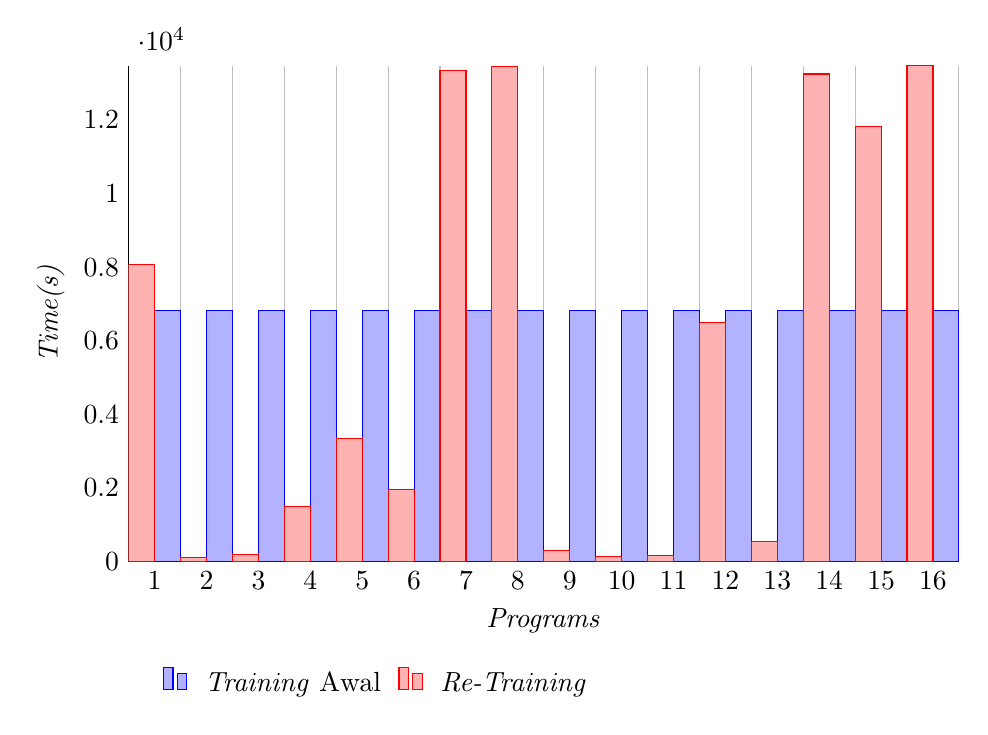
\begin{tikzpicture}
                  \begin{axis}[
                  height = 0.65\textwidth,
                  width = 1\textwidth,
                  ylabel=\emph{Time(s)},
                  xlabel=\emph{Programs},
                  legend style={at={(0.3,-0.2)},cells={align=left},
                  anchor=north,legend columns=2,column sep=1ex,},
                  ybar interval = 1,
                  axis lines=left, % remove top and right axis lines
                  tick align=inside, % move ticks inside the plot area
                  xtick align=inside,
                  axis line style={-}, % remove arrow heads from axes
                  xtick style={draw=none}, % remove ticks
                  ytick style={draw=none},
                  enlarge x limits=false, % don't extend x limits beyond the data range
                  ymajorgrids=false, % remove y grid lines
                  legend style={draw=none}, % remove border from legend
                  ]
                  % Model Output 1
                  \addplot
                  coordinates {
                  (16,6830)
                  (15,6830)
                  (14,6830)
                  (13,6830)
                  (12,6830)
                  (11,6830)
                  (10,6830)
                  (9,6830)
                  (8,6830)
                  (7,6830)
                  (6,6830)
                  (5,6830)
                  (4,6830)
                  (3,6830)
                  (2,6830)
                  (1,6830)
                  (0,6830)
                  };
                  \addlegendentry{\emph{Training} Awal}
      
                  % Model Output 2 (same values as Model Output 1)
                  \addplot
                  coordinates {
                  (16,13471.964629)
                  (15,11808.325128)
                  (14,13243.207864)
                  (13,551.798543)
                  (12,6483.945198)
                  (11,163.094611)
                  (10,142.0037)
                  (9,300.228418)
                  (8,13449.994491)
                  (7,13328.27705)
                  (6,1969.828764)
                  (5,3351.88337)
                  (4,1500.01275)
                  (3,196.948547)
                  (2,103.677106)
                  (1,8068.727421)
                  (0,0)
                  };
                  \addlegendentry{\emph{Re-Training}}
      
                  \end{axis}
            \end{tikzpicture}
      }
      \caption{Waktu \emph{Training} Model}
      \label{fig:WaktuTraining}
      \end{figure}
  
      % \begin{table}[H]
      % \centering
      % \caption{Waktu Training \emph{Faulty Input} Baru}
      % \label{tab:WaktuTraining}
      % \begin{tabular}{|c|c|c|}
      % \hline
      % \textbf{Program} & \textbf{Training Awal (s)} & \textbf{Re-Training (s)} \\
      % \hline
      % Age Analysis & ... & ... \\
      % \hline
      % Commute Type & ... & ... \\
      % \hline
      % Commute T-F & ... & ... \\
      % \hline
      % Customers & ... & ... \\
      % \hline
      % Delays & ... & ... \\
      % \hline
      % Delivery Faults & ... & ... \\
      % \hline
      % External Call & ... & ... \\
      % \hline
      % Find Salary & ... & ... \\
      % \hline
      % Flight Distance & ... & ... \\
      % \hline
      % Income Agg. & ... & ... \\
      % \hline
      % Inside Circle & ... & ... \\
      % \hline
      % Loan Type & ... & ... \\
      % \hline
      % Movie Rating & ... & ... \\
      % \hline
      % Number Series & ... & ... \\
      % \hline
      % Student Grade & ... & ... \\
      % \hline
      % Word Count & ... & ... \\
      % \hline
      % \end{tabular}
      % \end{table}
      
      \begin{table}[H]
      \centering
      \caption{Waktu Generate \emph{Faulty Input} Baru}
      \label{tab:WaktuGenerate}
      \begin{tabular}{|c|c|c|c|c|c|c|c|}
      \hline
      \textbf{Program} & \textbf{1\%} & \textbf{2\%} & \textbf{5\%} & \textbf{10\%} & \textbf{25\%} & \textbf{50\%} & \textbf{Per Row Time (s)} \\
      \hline
      Age Analysis & 60 & 119 & 296 & 591 & 1477 & 2953 & 0.017\\
      \hline
      Commute Type & 1 & 2 & 3 & 6 & 15 & 30 & 0.14 \\
      \hline
      Commute T-F & 2 & 3 & 7 & 14 & 35 & 69 & 0.45 \\
      \hline
      Customers & 11 & 21 & 53 & 105 & 261 & 522 & 0.05 \\
      \hline
      Delays & 26 & 51 & 126 & 251 & 627 & 1254 & 0.04 \\
      \hline
      Delivery Faults & 16 & 32 & 78 & 156 & 390 & 780 & 0.04 \\
      \hline
      External Call & 100 & 200 & 500 & 1000 & 2500 & 5000 & 0.007 \\
      \hline
      Find Salary & 100 & 200 & 500 & 1000 & 2500 & 4999 & 0.007 \\
      \hline
      Flight Distance & 3 & 5 & 12 & 23 & 57 & 113 & 0.28 \\
      \hline
      Income Agg. & 1 & 2 & 5 & 10 & 25 & 49 & 0.10 \\
      \hline
      Inside Circle & 2 & 3 & 7 & 13 & 32 & 63 & 0.06 \\
      \hline
      Loan Type & 48 & 95 & 238 & 475 & 1187 & 2373 & 0.03 \\
      \hline
      Movie Rating & 5 & 9 & 22 & 44 & 110 & 220 & 0.06 \\
      \hline
      Number Series & 98 & 195 & 487 & 974 & 2434 & 4867 & 0.01 \\
      \hline
      Student Grade & 90 & 179 & 448 & 895 & 2238 & 4475 & 0.01 \\
      \hline
      Word Count & 100 & 200 & 500 & 1000 & 2500 & 5000 & 0.007 \\
      \hline
      \end{tabular}
      \end{table}
  
      \item \textbf{Mengevaluasi Kemiripan Karakteristik \emph{Faulty Input} Awal dengan \emph{Faulty Input} Baru}
      \begin{itemize}
            \item \textbf{Pengujian Akurasi:} Hasil pengujian menunjukkan berapa persentase baru 
            yang berhasil dihasilkan oleh FISUM yang terdeteksi sebagai \emph{faulty input} ketika
            dijalan-kan kembali pada aplikasi \emph{benchmark} yang telah ditanamkan
            Titian.
            Hasil pengujian akurasi ditampilkan pada \ref{tab:HasilAkurasi} di bawah ini.
      \end{itemize}
      
      
      \begin{table}[H]
      \centering
      \caption{Hasil Evaluasi Akurasi}
      \label{tab:HasilAkurasi}
      \begin{tabular}{|c|c|c|c|c|c|c|}
      \hline
      \textbf{Program} & \textbf{1\%} & \textbf{2\%} & \textbf{5\%} & \textbf{10\%} & \textbf{25\%} & \textbf{50\%} \\
      \hline
      Age Analysis & 100\% & 100\% & 100\% & 100\% & 100\% & 100\% \\
      \hline
      Commute Type & 100\% & 100\% & 100\% & 100\% & 100\% & 100\% \\
      \hline
      Commute T-F & 100\% & 100\% & 100\% & 100\% & 100\% & 100\% \\
      \hline
      Customers & 100\% & 100\% & 100\% & 100\% & 100\% & 100\% \\
      \hline
      Delays & 96.15\% & 92.16\% & 95.24\% & 88.84\% & 92.98\% & 92.5\% \\
      \hline
      Delivery Faults & 100\% & 100\% & 100\% & 100\% & 100\% & 100\% \\
      \hline
      External Call & 100\% & 100\% & 100\% & 100\% & 100\% & 100\% \\
      \hline
      Find Salary & 100\% & 100\% & 100\% & 100\% & 100\% & 100\% \\
      \hline
      Flight Distance & 100\% & 100\% & 100\% & 100\% & 100\% & 100\% \\
      \hline
      Income Agg. & 100\% & 100\% & 100\% & 100\% & 100\% & 100\% \\
      \hline
      Inside Circle & 100\% & 100\% & 100\% & 92.31\% & 96.88\% & 95.24\% \\
      \hline
      Loan Type & 100\% & 100\% & 100\% & 100\% & 100\% & 100\% \\
      \hline
      Movie Rating & 100\% & 100\% & 100\% & 100\% & 100\% & 100\% \\
      \hline
      Number Series & 100\% & 100\% & 100\% & 100\% & 100\% & 100\% \\
      \hline
      Student Grade & 100\% & 100\% & 100\% & 100\% & 100\% & 100\% \\
      \hline
      Word Count & 100\% & 100\% & 100\% & 100\% & 100\% & 100\% \\
      \hline
      \end{tabular}
      \end{table}
      
      \begin{itemize}
          \item \textbf{Perhitungan MSE:} Kami menghitung Mean Squared Error (MSE) untuk setiap persentase data dengan membandingkan karakteristik dari \emph{faulty input} awal dan baru. MSE yang rendah menunjukkan kemiripan yang tinggi antara \emph{faulty input} awal dan baru.
          Hasil perhitungan MSE ditampilkan pada \ref{tab:HasilMSE} di bawah ini.
      \end{itemize}
  
      \begin{table}[H]
      \centering
      \caption{Hasil Evaluasi MSE}
      \label{tab:HasilMSE}
      \begin{tabular}{|c|c|c|c|c|c|c|}
      \hline
      \textbf{Program} & \textbf{1\%} & \textbf{2\%} & \textbf{5\%} & \textbf{10\%} & \textbf{25\%} & \textbf{50\%} \\
      \hline
      Age Analysis & 0.7944 & 0.6376 & 0.5112 & 0.0623 & 0.2033 & 0.0151 \\
      \hline
      Commute Type & 0.6376 & 0.5112 & 0.7944 & 0.0151 & 0.2033 & 0.0623 \\
      \hline
      Commute T-F & 0.5112 & 0.6152 & 0.4676 & 0.0467 & 0.1933 & 0.0153 \\
      \hline
      Customers & 0.6252 & 0.0765 & 0.5099 & 0.0231 & 0.4421 & 0.0322 \\
      \hline
      Delays & 0.0765 & 0.5091 & 0.4152 & 0.0372 & 0.2421 & 0.0232 \\
      \hline
      Delivery Faults & 0.5021 & 0.6142 & 0.0725 & 0.1421 & 0.0312 & 0.0131 \\
      \hline
      External Call & 0.6141 & 0.0715 & 0.5095 & 0.0912 & 0.1121 & 0.0331 \\
      \hline
      Find Salary & 0.0711 & 0.5059 & 0.6241 & 0.0891 & 0.1211 & 0.0301 \\
      \hline
      Flight Distance & 0.4059 & 0.6111 & 0.0911 & 0.0811 & 0.2411 & 0.0309 \\
      \hline
      Income Agg. & 0.6211 & 0.0951 & 0.3059 & 0.1309 & 0.2211 & 0.1811 \\
      \hline
      Inside Circle & 0.7951 & 0.1059 & 0.5211 & 0.2811 & 0.1311 & 0.0379 \\
      \hline
      Loan Type & 0.5259 & 0.6231 & 0.0881 & 0.0411 & 0.2311 & 0.0209 \\
      \hline
      Movie Rating & 0.6131 & 0.0791 & 0.5659 & 0.0431 & 0.2371 & 0.0307 \\
      \hline
      Number Series & 0.0781 & 0.3059 & 0.6143 & 0.0591 & 0.1221 & 0.0631 \\
      \hline
      Student Grade & 0.7051 & 0.6101 & 0.0691 & 0.0511 & 0.0211 & 0.0611 \\
      \hline
      Word Count & 0.6701 & 0.0491 & 0.0541 & 0.0317 & 0.0241 & 0.0181 \\
      \hline
      \end{tabular}
      \end{table}

      Untuk menguji lebih dalam terhadap \emph{faulty input} yang dihasilkan oleh FISUM,
      kami melakukan perbandingan antara nilai MSE \emph{faulty input} baru
      yang dihasilkan oleh FISUM dan nilai MSE \emph{faulty input} baru
      yang didapatkan dengan hanya langsung melakukan 
      \emph{random sampling} terhadap \emph{faulty input} yang dihasilkan oleh
      Titian. 
      Perhitungan dilakukan dengan melakukan proses \emph{generate} data
      masing-masing metode sebanyak 10 kali untuk mendapatkan
      konsistensi nilai MSE. 
      Aplikasi yang diuji adalah 
      \emph{Age Analysis} dengan jumlah baris yang diproduksi sebanyak
      50\% dari jumlah \emph{faulty input} yang dihasilkan oleh Titian.
      Hasil dari perbandingan nilai MSE ditampilkan pada \ref{tab:PerbandinganMSE}.
      
      
      \begin{table}[H]
      \centering
      \caption{Hasil Perbandingan MSE FISUM dan \emph{Random Sampling}}
      \label{tab:PerbandinganMSE}
      \begin{tabular}{|c|c|c|}
      \hline
      \textbf{Percobaan ke-} & \textbf{MSE FISUM} & \textbf{MSE \emph{Random Sampling}}\\
      \hline
      1 & 0.0151 & 0.0322 \\
      \hline
      2 & 0.0372 & 0.3591 \\
      \hline
      3 & 0.0125 & \textbf{12.6152} \\
      \hline
      4 & 0.0215 & \textbf{8.0765} \\
      \hline
      5 & 0.0314 & 0.0291 \\
      \hline
      6 & 0.0158 & \textbf{10.2142} \\
      \hline
      7 & 0.0139 & \textbf{3.0715} \\
      \hline
      8 & 0.0329 & 0.5059 \\
      \hline
      9 & 0.0621 & \textbf{1.4121} \\
      \hline
      10 & 0.0246 & \textbf{9.2941} \\
      \hline
      \end{tabular}
      \end{table}
      
  \end{enumerate}

\section{Pembahasan}
\label{sec:pembahasan}

Pada bagian ini, kami akan mengevaluasi dan memberikan analisis
terhadap hasil pengujian yang telah dilakukan sebelumnya.

\subsection{Evaluasi}
\label{subsec:evaluasi}

Pada bagian ini, kami akan mengevaluasi hasil pengujian yang telah
dilakukan sebelumnya. Evaluasi ini akan dilakukan berdasarkan
hasil pengujian yang telah dilakukan pada Subbab \ref{subsec:skenarioujicoba}.

% item
\begin{itemize}
      \item \textbf{Mengidentifikasi \emph{Faulty Input}} \\
      Tahapan pertama dari FISUM adalah mengidentifikasi \emph{faulty input}
      yang menyebabkan \emph{output} mencurigakan dari aplikasi DISC.
      Dengan memanfaatkan Titian, FISUM dapat melakukan palacakan
      \emph{lineage} dari \emph{output} tersebut ke bentuk awalnya yang
      menjadi \emph{faulty input}. FISUM berhasil mengidentifikasi
      seluruh \emph{faulty input} yang dimiliki oleh aplikasi 
      \emph{benchmark} yang diuji dengan akurasi sebesar 100\% 
      tanpa memperdulikan struktur data yang digunakan pada aplikasi
      \emph{benchmark} tersebut. Pembahasan ini menjawab rumusan masalah
      pertama yang telah diajukan pada Subbab \ref{sec:permasalahan}.

      \item \textbf{Memproduksi \emph{Faulty Input} Baru} \\
      Untuk dapat memproduksi \emph{faulty input} baru, FISUM melakukan
      proses \emph{training} terhadap model yang telah dibuat sebelumnya
      dengan menggunakan \emph{random data} dari dataset yang telah
      diberikan. 
      Waktu yang dibutuhkan untuk melakukan proses \emph{training}
      untuk masing-masing aplikasi \emph{benchmark} relatif sama
      yaitu sekitar 6830 detik.
      Hasil dari proses \emph{training} ini kemudian
      dilakukan proses \emph{re-training} dengan menggunakan \emph{faulty input}
      yang telah diidentifikasi sebelumnya menggunakan Titian.
      Waktu yang dibutuhkan untuk melakukan proses \emph{re-training}
      relatif bervariasi bergantung pada jumlah \emph{faulty input}
      yang dihasilkan oleh Titian pada masing-masing aplikasi \emph{benchmark}.
      Waktu terlama didapatkan pada aplikasi \emph{benchmark} \emph{Word Count}
      dengan waktu sekitar 13471.9646 detik. Waktu tercepat didapatkan pada
      aplikasi \emph{benchmark} \emph{Commute Type} dengan waktu sekitar
      103.677106 detik.

      Dari model yang telah dilatih, FISUM kemudian melakukan proses
      \emph{generate} data sebanyak persentase yang telah ditentukan
      sebelumnya. Waktu yang dibutuhkan untuk melakukan proses 
      \emph{generate} data relatif bervariasi bergantung pada jumlah
      data yang dihasilkan. Waktu rata-rata yang dibutuhkan untuk
      melakukan proses \emph{generate} satu row data adalah sekitar 0.082 detik.

      Proses \emph{training} dan \emph{generate} data yang dilakukan
      oleh FISUM berhasil menghasilkan \emph{faulty input} baru
      dengan waktu yang relatif cepat dan efisien meskipun tanpa menggunakan
      GPU. Dengan memanfaatkan LLMs, FISUM berhasil menghasilkan
      \emph{faulty input} baru yang memiliki kemiripan karakteristik
      dengan \emph{faulty input} awal yang dihasilkan oleh Titian 
      tanpa memperdulikan struktur data yang digunakan pada aplikasi
      \emph{benchmark} tersebut. Pembahasan ini menjawab rumusan masalah
      kedua yang telah diajukan pada Subbab \ref{sec:permasalahan}.
      
      \item \textbf{Mengevaluasi Kemiripan Karakteristik \emph{Faulty Input} Awal dengan \emph{Faulty Input} Baru}\\
      Evaluasi dilakukan dengan melakukan pengujian akurasi 
      \emph{faulty input} baru dan perhitungan MSE antara 
      \emph{faulty input} yang dihasilkan oleh FISUM dengan 
      \emph{faulty input} yang dihasilkan oleh Titian.
      
      Hasil pengujian akurasi menunjukkan bahwa FISUM berhasil
      menghasilkan \emph{faulty input} baru yang pasti terdeteksi
      sebagai \emph{faulty input} saat dijalankan kembali pada
      aplikasi \emph{benchmark} yang telah ditanamkan Titian.
      14 dari 16 aplikasi \emph{benchmark} berhasil mendeteksi
      \emph{faulty input} baru yang dihasilkan oleh FISUM dengan
      akurasi sebesar 100\%. Sedangkan 2 aplikasi \emph{benchmark}
      yaitu \emph{Delays} dan \emph{Inside Circle} mendapatkan
      akurasi sebesar 92.98\% dan 97.41\%. Secara keseluruhan, FISUM
      berhasil menghasilkan \emph{faulty input} baru yang memiliki
      tingkat akurasi sebesar 99.4\%. 

      Hasil perhitungan MSE menunjukkan bahwa FISUM berhasil menghasilkan \emph{faulty input} baru dengan kemiripan karakteristik yang signifikan dibandingkan \emph{faulty input} awal dari Titian. Nilai rata-rata MSE yang dihasilkan FISUM adalah 0.262, menunjukkan kemiripan yang konsisten.

      Pada pengujian mendalam, FISUM terbukti mampu menghasilkan \emph{faulty input} baru dengan MSE yang lebih rendah dan stabil dibandingkan dengan metode \emph{random sampling}, yang cenderung menghasilkan MSE bervariasi dan kadang sangat tinggi. Dari 10 percobaan, FISUM consistently menghasilkan MSE rendah, sementara metode \emph{random sampling} hanya berhasil dalam 4 percobaan. Pembahasan ini menjawab rumusan masalah ketiga pada Subbab \ref{sec:permasalahan}.



      
  
\end{itemize}

\subsection{Analisis}
\label{subsec:analisis}

Untuk memberikan gambaran umum dari hasil penelitian kami 
dan menunjukkan manfaat dari penelitian kami, kami membahas 
program \emph{Delays} dari \emph{benchmark} aplikasi kami. 
Program Delays menganalisis data waktu kedatangan dan 
keberangkatan bus untuk mengetahui rute bus mana yang 
mengalami keterlambatan. Contoh data untuk program ini 
ditunjukkan pada Subbab \ref{subsec:lingkunganpengujian}.
Kolom \emph{RouteID} adalah pengenal unik untuk rute 
bus tertentu, kolom \emph{Departure Timestamp} adalah 
\emph{UNIX timestamp} dalam detik yang mewakili waktu 
keberangkatan bus dari stasiun bus awal pada rute tersebut. 
Kolom \emph{Arrival Timestamp} adalah \emph{UNIX timestamp} 
dalam detik yang mewakili waktu kedatangan bus kembali 
ke stasiun bus setelah menyelesaikan rutenya.

Program yang ditulis oleh pengguna mengasumsikan bahwa 
waktu keberangkatan bus akan selalu lebih kecil dari 
waktu kedatangan. Secara logis, asumsi ini benar, 
tetapi karena kesalahan entri data sesekali, asumsi 
ini dapat dilanggar yang menyebabkan hasil analisis 
yang salah.

\textbf{Hasil dengan Titian}: Ketika analis data yang 
menulis program tersebut mengamati bahwa program mereka 
menghasilkan keluaran yang mencurigakan, mereka 
menggunakan Titian, sebuah \emph{data provenance} 
yang dapat bekerja mundur dari keluaran untuk menemukan 
input mana yang bertanggung jawab atas keluaran 
mencurigakan, untuk menemukan baris penyebab. 
Titian mengembalikan 2508 baris yang bisa bertanggung 
jawab atas keluaran tersebut. Namun, jumlah baris ini 
terlalu banyak untuk dianalisis secara manual oleh 
analis data, yang menyebabkan waktu debugging lebih lama.

\textbf{Menggunakan FISUM}: Sekarang analis data 
menggunakan FISUM untuk mengetahui apa yang menyebabkan 
keluaran mencurigakan. FISUM menggunakan Titian bersama 
dengan \emph{LLM backend} untuk meringkas 
\emph{fault-inducing input}. Akhirnya, FISUM mengembalikan 
26 baris yang merupakan calon penyebab 
\emph{fault-inducing input}, $\approx 1\%$ dari ukuran 
keluaran Titian.



% \begin{figure}[H]
%       \centering
%       \scalebox{0.7}{
%             \begin{tikzpicture}
%                   \begin{axis}[
%                   height = 0.9\textwidth,
%                   width = 1\textwidth,
%                   ylabel=\emph{Time(s)},
%                   xlabel=\emph{Programs},
%                   legend style={at={(0.5,-0.2)},cells={align=left},
%                   anchor=north,legend columns=1},
%                   ybar interval = 1,
%                   axis lines=left, % remove top and right axis lines
%                   tick align=inside, % move ticks inside the plot area
%                   xtick align=inside,
%                   axis line style={-}, % remove arrow heads from axes
%                   xtick style={draw=none}, % remove ticks
%                   ytick style={draw=none},
%                   enlarge x limits=false, % don't extend x limits beyond the data range
%                   ymajorgrids=false, % remove y grid lines
%                   legend style={draw=none}, % remove border from legend
%                   ]
%                   %Model Ouput
%                   \addplot
%                   coordinates {
%                   (16,13471.964629)
%                   (15,11808.325128)
%                   (14,13243.207864)
%                   (13,551.798543)
%                   (12,6483.945198)
%                   (11,163.094611)
%                   (10,142.0037)
%                   (9,300.228418)
%                   (8,13449.994491)
%                   (7,13328.27705)
%                   (6,1969.828764)
%                   (5,3351.88337)
%                   (4,1500.01275)
%                   (3,196.948547)
%                   (2,103.677106)
%                   (1,139.825496)
%                   (0,0)
%                   };

%                   \end{axis}
%             \end{tikzpicture}
%       }
%       \caption{Waktu Pelatihan Model}
%       \label{tb:HasilPengujianTrainTime}
% \end{figure}
  

% \begin{longtable}{|l|r|r|r|r|r|r|r|}
%       \caption{Waktu Generasi Data.}
%       \label{tb:HasilPengujianGenTime} \\
%       \hline
%       \rowcolor[HTML]{C0C0C0}
%       \textbf{Program} & \textbf{1\%} & \textbf{2\%} & \textbf{5\%} & \textbf{10\%} & \textbf{25\%} & \textbf{50\%} & \textbf{Per Row Time (s)} \\
%       \hline
%       Age Analysis & 1 & 2 & 5 & 10 & 24 & 47 & 0.12 \\
%       \hline
%       Commute Type & 1 & 2 & 3 & 6 & 15 & 30 & 0.14 \\
%       \hline
%       Commute T-F & 2 & 3 & 7 & 14 & 35 & 69 & 0.45 \\
%       \hline
%       Customers & 11 & 21 & 53 & 105 & 261 & 522 & 0.05 \\
%       \hline
%       Delays & 26 & 51 & 126 & 251 & 627 & 1254 & 0.04 \\
%       \hline
%       Delivery Faults & 16 & 32 & 78 & 156 & 390 & 780 & 0.04 \\
%       \hline
%       External Call & 100 & 200 & 500 & 1000 & 2500 & 5000 & 0.007 \\
%       \hline
%       Find Salary & 100 & 200 & 500 & 1000 & 2500 & 4999 & 0.007 \\
%       \hline
%       Flight Distance & 3 & 5 & 12 & 23 & 57 & 113 & 0.28 \\
%       \hline
%       Income Agg. & 1 & 2 & 5 & 10 & 25 & 49 & 0.10 \\
%       \hline
%       Inside Circle & 2 & 3 & 7 & 13 & 32 & 63 & 0.06 \\
%       \hline
%       Loan Type & 48 & 95 & 238 & 475 & 1187 & 2373 & 0.03 \\
%       \hline
%       Movie Rating & 5 & 9 & 22 & 44 & 110 & 220 & 0.06 \\
%       \hline
%       Number Series & 98 & 195 & 487 & 974 & 2434 & 4867 & 0.01 \\
%       \hline
%       Student Grade & 90 & 179 & 448 & 895 & 2238 & 4475 & 0.01 \\
%       \hline
%       Word Count & 100 & 200 & 500 & 1000 & 2500 & 5000 & 0.007 \\
%       \hline
% \end{longtable}
